% 1960 年全国卷第 5 题：钢珠测量机件小孔直径。
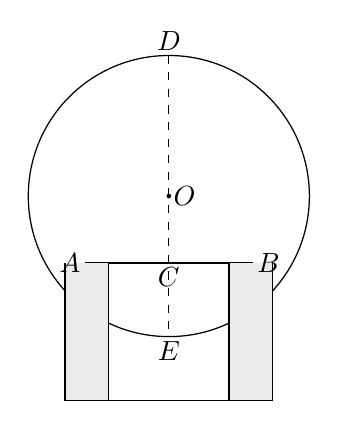
\begin{tikzpicture}[scale=0.85, line width=0.45pt,
  every node/.style={inner sep=1.5pt}]
  \coordinate (O) at (0,1.7);
  \coordinate (D) at (0,3.8);
  \coordinate (E) at (0,-0.4);
  \coordinate (C) at (0,0.7);
  \coordinate (A) at (-1.25,0.7);
  \coordinate (B) at (1.25,0.7);
  \draw (O) circle (2.1);
  \draw[dashed] (D)--(E);
  \draw (A)--(B);
  \draw[dashed] (A)--(C)--(B);
  \draw[fill=gray!15] (-1.55,0.7)--(-1.55,-1.35)--(-0.9,-1.35)--(-0.9,0.7);
  \draw[fill=gray!15] (0.9,0.7)--(0.9,-1.35)--(1.55,-1.35)--(1.55,0.7);
  \draw (-0.9,-1.35)--(0.9,-1.35);
  \fill (O) circle (0.035);
  \node[anchor=south] at (D) {$D$};
  \node[anchor=west] at (O) {$O$};
  \node[anchor=north] at (C) {$C$};
  \node[anchor=east] at (A) {$A$};
  \node[anchor=west] at (B) {$B$};
  \node[anchor=north] at (E) {$E$};
\end{tikzpicture}
